\documentclass[10pt]{article}         %% What type of document you're writing.

%%%%% Preamble

%% Packages to use

\usepackage{amsmath,amsfonts,amssymb,url}   %% AMS mathematics macros
\usepackage[numbers,sort&compress]{natbib}
\usepackage{graphicx}
\usepackage{subcaption}
\usepackage[svgnames]{xcolor}
\usepackage{listings}
\usepackage{placeins}
\usepackage{afterpage}
\usepackage{float}

\graphicspath{ {./images/} }
%% Title Information.

%\textsc{\newenvironment{changemargin}[2]{%
%\begin{list}{}{%
%\setlength{\topsep}{0pt}%
%\setlength{\leftmargin}{#1}%
%\setlength{\rightmargin}{#2}%
%\setlength{\listparindent}{\parindent}%
%\setlength{\itemindent}{\parindent}%
%\setlength{\parsep}{\parskip}%
%}%
%\item[]}{\end{list}}}

\lstset{language=R,
    basicstyle=\small\ttfamily,
    stringstyle=\color{DarkGreen},
    otherkeywords={0,1,2,3,4,5,6,7,8,9},
    morekeywords={TRUE,FALSE},
    deletekeywords={data,frame,length,as,character},
    keywordstyle=\color{blue},
    commentstyle=\color{DarkGreen},
}

\title{Comparison of survivals in control and exposed populations and its implications for virulence}
\author{Petr Kouba}
%% \date{1 July 2004}           %% By default, LaTeX uses the current date

%%%%% The Document

\begin{document}
\maketitle

This document summarizes the differences between deathrate of exposed and control populations and provides the virulence taken with respect to the mortality of the control population. For the purpose of the whole document by "exposed" population, we mean the population which was exposed to the infection, but did not get infected.

\newpage
\section{Survival in the control population versus survival in the exposed population}


\begin{figure}[H]
\begin{subfigure}[b]{0.6\textwidth}
    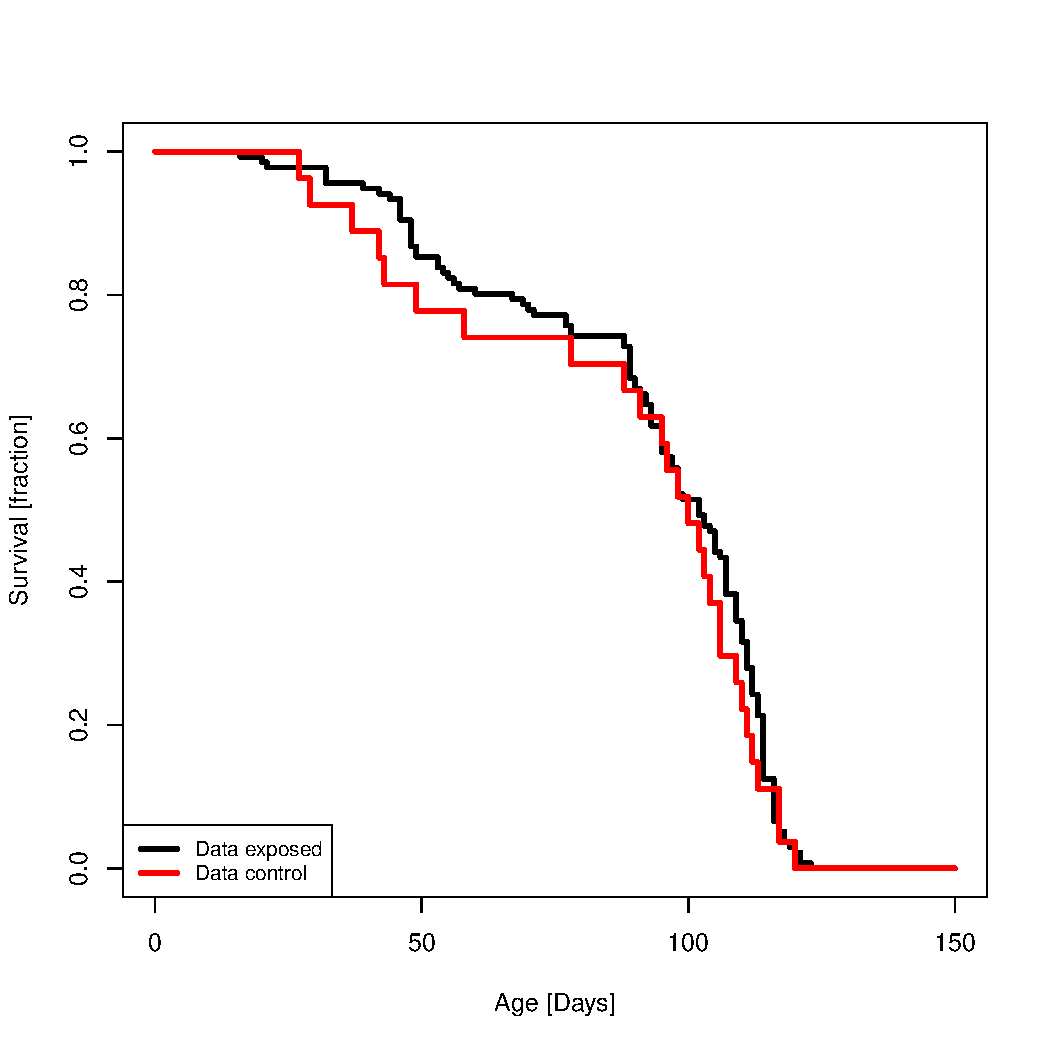
\includegraphics[width=\textwidth]{Survival_exposed_versus_control.pdf}
    \caption{Survival of whole exposed [136Daphnias] and control [27Daphnia] populations, regardless of the age at infection.}
    \label{fig:subfigure_1}
  \end{subfigure}
  %
  \begin{subfigure}[b]{0.6\textwidth}
    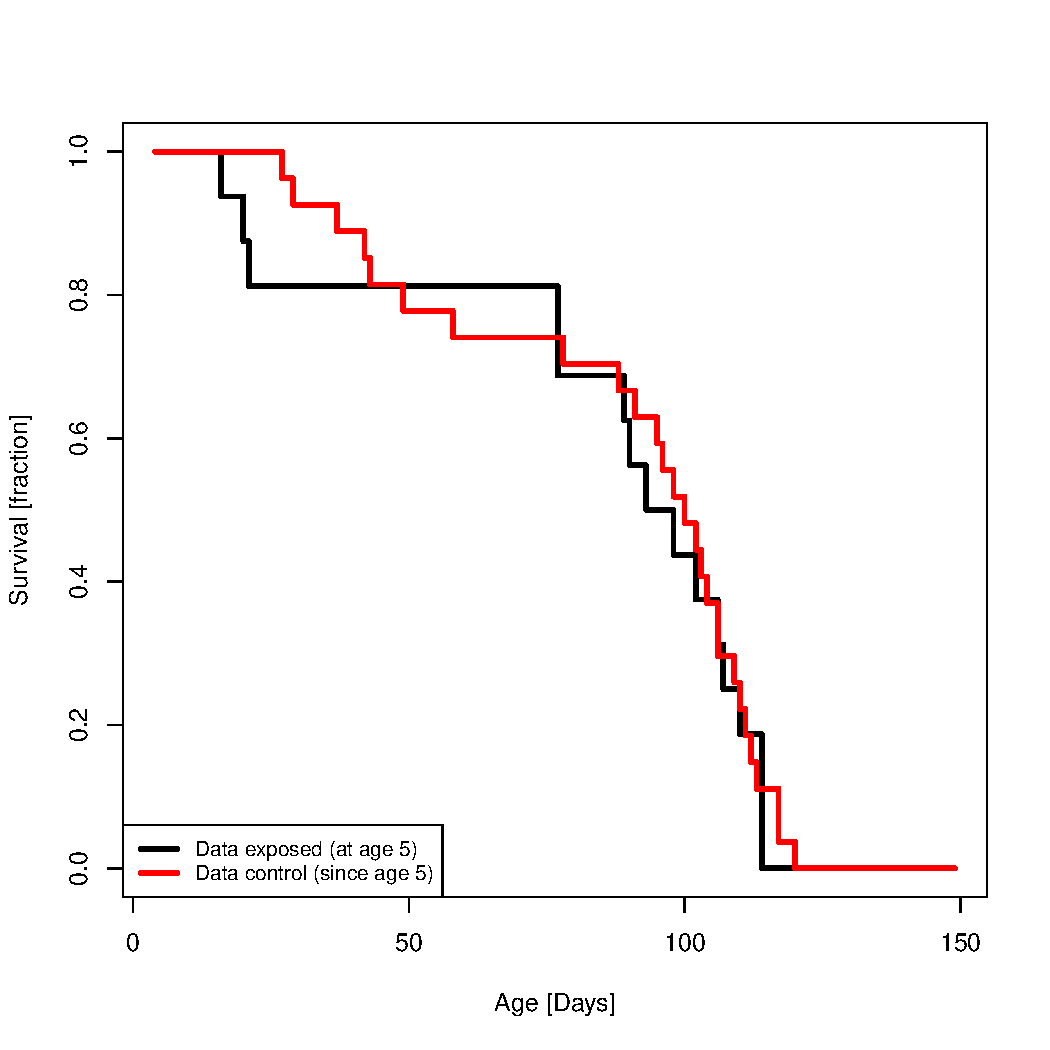
\includegraphics[width=\textwidth]{Survival_data_aai_5.pdf}
    \caption{Survival of population exposed at age 5 [16Daphnias] and control population since age 5 [27Daphnias].}
    \label{fig:subfigure_2}
  \end{subfigure}
  \begin{subfigure}[b]{0.6\textwidth}
    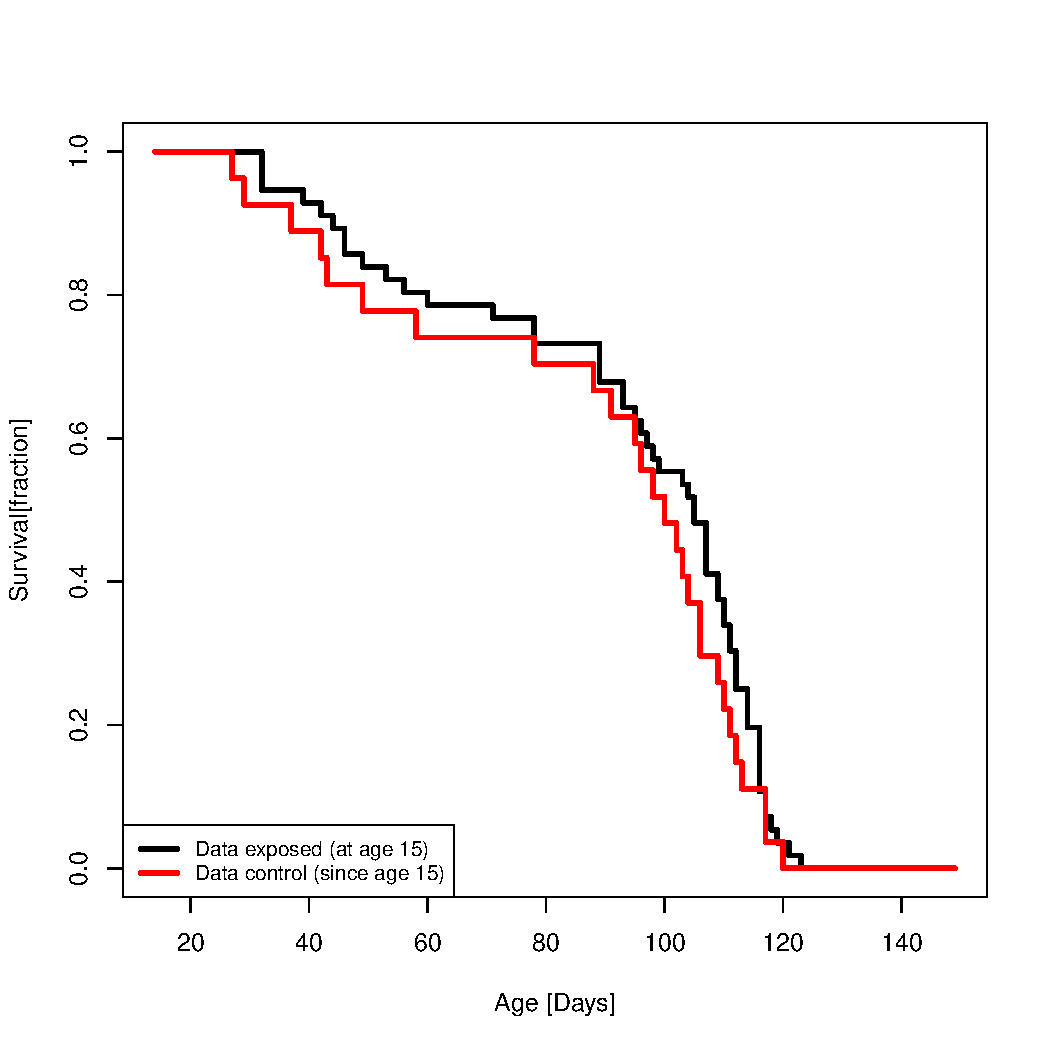
\includegraphics[width=\textwidth]{Survival_data_aai_15.pdf}
    \caption{Survival of population exposed at age 15 [56Daphnias] and control population since age 15 [27Daphnias].}
    \label{fig:subfigure_3}
  \end{subfigure}
  %
  \begin{subfigure}[b]{0.6\textwidth}
    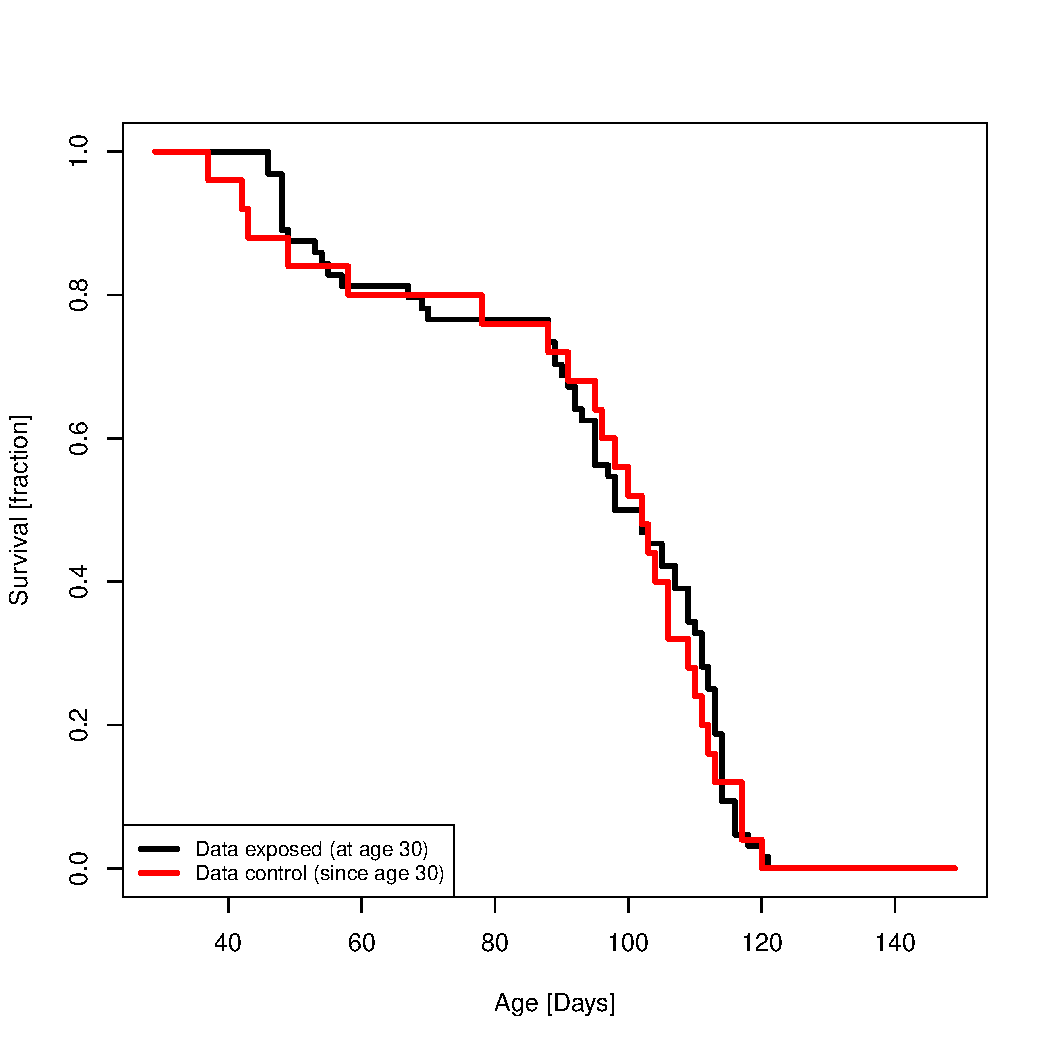
\includegraphics[width=\textwidth]{Survival_data_aai_30.pdf}
    \caption{Survival of population exposed at age 30 [64Daphnias] and control population since age 30 [25Daphnias].}
    \label{fig:subfigure_4}
  \end{subfigure}
  \caption{Comparison of survival in exposed and control populations, within compartments based on ages at infection}
  \label{survivals_exp_control}
\end{figure}

From the plots in Figure~\ref{survivals_exp_control}, we can see that the survival pattern is very similar in control and exposed populations, except for age at infection 15, where there is a discrepancy. This discrepancy could be however a result of a small sample size in the exposed population for that given age at infection. Lets try to verify the similarity of these survival distributions statistically.

\subsection{Hypothesis testing of the sameness of the exposed and control survival distributions}

\subsubsection{Kolmogorov-Smirnov test}
As a first test, we tried the Kolmogorov-Smirnov test. Choosing critical p-value to be $p=0.05$, we got rejection of the null hypothesis for the group belonging to the age at infection 5 ($p=0.009 $). For ages at infection 15 ($p=0.057$) and 30 ($p=0.699$), the null hypothesis (both distributions being drawn from the same distribution) was accepted.

Apperently, the Kolmogorov-Smirnov test might be too harsh on discrete data samples. Therefore we proceeded, by looking for further tests.\newline\newline
\textcolor{red}{Question: What other tests might be convenient for our case?}

\subsection{Sample sizes for exposed and control populations}

If we would assume that the exposed and the control populations follow the same survival distribution (which was confirmend by Kolmogorov-Smirnov test in two age-at-infection-groups out of 3), we could take the deathrate of the control population as the reference deathrate in all three age-at-infection classes and compute the virulence using this natural deathrate.
	However, the control population only contained 27 individuals, which only exceeds the sample size of population exposed at age 5 (16 individuals). Whereas the populations exposed at age 15 (56 individuals) and at age 30 (64 individuals) both provide us with larger sample.
	
As for the question regarding the sample sizes you had last time: "Why does the overall sample size (exposed +infected) decrease with age at infection? Does it correspond to the deathrate?"

Our samples have the following numbers of individuals:
$Infected_{at age 5} + Exposed_{at age 5} = 113$
$Infected_{at age 15} + Exposed_{at age 15} = 83$
$Infected_{at age 30} + Exposed_{at age 30} = 78$

Whereas if we would start with 113, who survived age 5 in each compartment, reflecting the deathrate we would get the sample sizes of 113, 113 and 105 respectively. So I believe this decrease is due to the design of the experiment and I do not see a good reason for it.

\textcolor{red}{Question: If we manage to show that the population exposed at age 5 and the control population follow the same distribution (by using a better suited test), can we just - in order to get the largest sample possible - merge all of the exposed individuals and control into one compartment of uninfecteds and use this whole compartment for the estimation of the natural deathrate? And if we find difference in exposing the individuals age 5, could we just estimate 2 different natural deathrates?(one for the exposed at age 5 and one common for the rest) }

\subsection{Fitting survival for "exposed population" and "uninfected population"}

\begin{figure}[H]
\begin{subfigure}[b]{0.6\textwidth}
    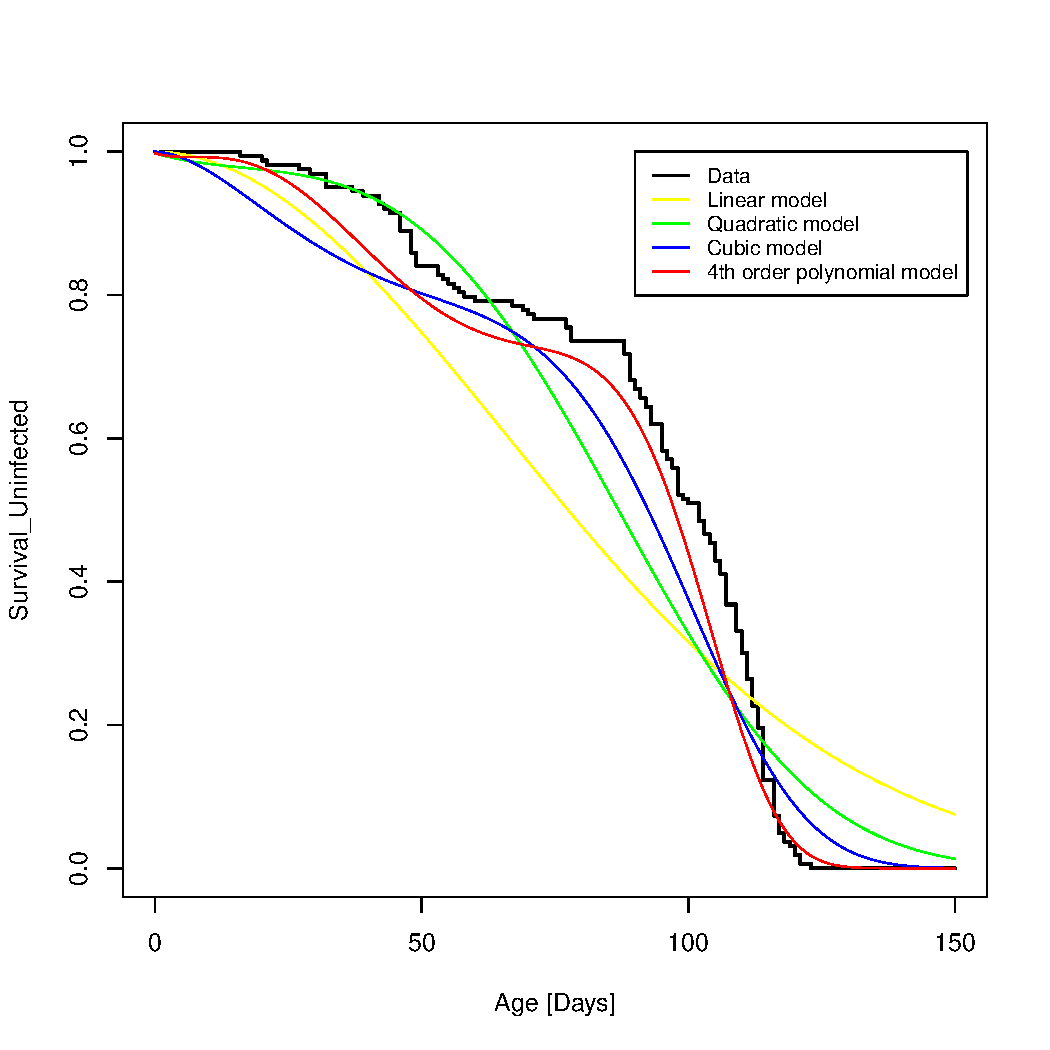
\includegraphics[width=\textwidth]{uninfected_population_survival_and_fit.pdf}
    \caption{Survival of the uninfected population and the corresponding fits}
    \label{fig:subfigure_exp}
  \end{subfigure}
  %
  \begin{subfigure}[b]{0.6\textwidth}
    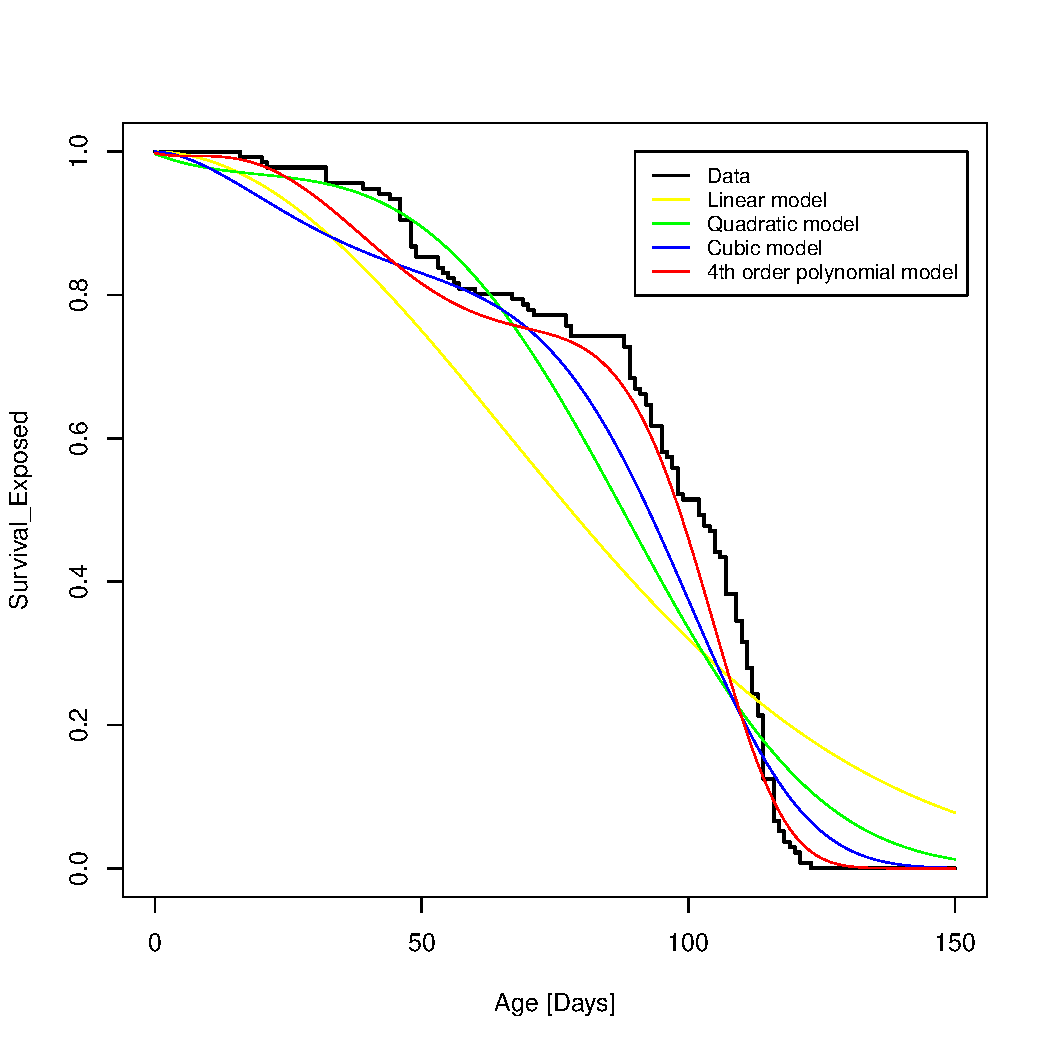
\includegraphics[width=\textwidth]{exposed_population_survival_and_fit.pdf}
    \caption{Survival of the exposed population and the corresponding fits}
    \label{fig:subfigure_uninfected}
  \end{subfigure}
  \caption{Comparison of survival in exposed and uninfected populations}
  \label{survivals_exp_uninfected}
\end{figure}

\section{Virulences with respect to the chosen reference deathrate}

\textcolor{blue}{TODO: As soon as we decide on which compartment(s) to use for the estimation of the natural death rate, I will put the updated virulences here}

\textcolor{blue}{TODO: Examine the statistical significance of the differences in virulence between different ages at infection}

\textcolor{red}{What would be the proper way to try to prove the significant difference between virulences for different ages at infection? Could logrank test be applied on the survival distribution models generated by the different virulences?}



\bibliographystyle{unsrtnat}
\bibliography{bibliography_SIE_model}

\end{document}


